% CVPR 2026 Paper Template; see https://github.com/cvpr-org/author-kit
\documentclass[10pt,twocolumn,letterpaper]{article}
\usepackage{cvpr} 

%% This file contains a number of tweaks that are typically applied to the main document.
%% They are not enabled by default, but can be enabled by uncommenting the relevant lines.

%%
%% Inline annotations; for predefined colors, refer to "dvipsnames" in the xcolor package:
%% https://tinyurl.com/overleaf-colors
%%
\newcommand{\red}[1]{{\color{red}#1}}
\newcommand{\todo}[1]{{\color{red}#1}}
\newcommand{\TODO}[1]{\textbf{\color{red}[TODO: #1]}}
%%
%% disable for camera ready / submission by uncommenting these lines  
%%
% \renewcommand{\TODO}[1]{}
% \renewcommand{\todo}[1]{#1}

%%
%% work harder in optimizing text layout. Typically shrinks text by 1/6 of page, enable
%% it at the very end of the writing process, when you are just above the page limit
%%
% \usepackage{microtype}

%%
%% fine-tune paragraph spacing
%%
% \renewcommand{\paragraph}[1]{\vspace{.5em}\noindent\textbf{#1.}}

%%
%% globally adjusts space between figure and caption
%%
% \setlength{\abovecaptionskip}{.5em}


%%
%% Allows "the use of \paper to refer to the project name"
%% with automatic management of space at the end of the word
%%
% \usepackage{xspace}
% \newcommand{\paper}{ProjectName\xspace}

%%
%% Commonly used math definitions
%%
% \DeclareMathOperator*{\argmin}{arg\,min}
% \DeclareMathOperator*{\argmax}{arg\,max}

%%
%% Tigthen underline
%%
% \usepackage{soul}
% \setuldepth{foobar}

\definecolor{cvprblue}{rgb}{0.21,0.49,0.74}
\usepackage[pagebackref,breaklinks,colorlinks,allcolors=cvprblue]{hyperref}

%%%%%%%%% PAPER ID
\def\paperID{1}
\def\confName{5031}
\def\confYear{2026}

%%%%%%%%% AUTHORS
\author{
Rania Haas \quad Matthew Goldsberry \quad Nhat Pham\\
University of Cincinnati\\
Cincinnati, OH, USA\\
{\tt\small \{haasr3, goldsbme, phamn2\}@mail.uc.edu}
}

%%%%%%%%% TITLE
\title{StateFarm Distracted Driver Detection Model}

\begin{document}
\maketitle
% Page budget. The limit is 6 pages for CS5131 and 8 for CS6031, counted from the title to the
% end of the closing statements. The references do not count toward the limit, so the
% bibliography may run onto page 7 (or 9) and beyond. Everything above the bibliography counts,
% including the Reproducibility and AI Tool Disclosure statements.
% Sizes below are full pages (both columns) and sum to about 6. For 8 pages, grow Related Work
% (12 to 15 papers with a critical comparison), Experiments, and Error Analysis first.
%   Abstract + Introduction 0.75 | Related Work 0.75 | Dataset and Split 0.6 | Method 1.0
%   Experiments 1.6 | Error Analysis 0.8 | Discussion 0.35 | Conclusion 0.15 | Statements 0.15
% Main-body figures and tables (about 7): model diagram, main results table (with classical
% rows), leakage figure or table, scaling figure (fig14), failure cases with Grad-CAM
% (fig11b/11c), confusion matrix of the final model (fig09 or fig15), SOTA table (small).
\begin{abstract}
Approached with the task of detecting distracted drivers, we studied image-based distracted driver detection models on the State Farm Distracted Driver Detection (SFDDD) dataset, viewing several images from the dashboard including: safe driving, texting, phone calls, and reaching behind the passenger seat.
Distracted driving is a leading cause of road accidents, and automated in-cabin monitoring could enable timely driver alerts. 
We trained and fine tuned models from Kaggle's competition using [methods], and we evaluated with a driver-disjoint 70-30 test split.
Our best model achieves an accuracy of [X\%].
Denote about errors
These results suggest 
\end{abstract}



\section{Introduction}
\label{sec:intro}

One of the largest issues within driving is collions due to distracted drivers.
In 2024, over 300,000 US drivers were injured due to distracted drivers\cite{nhstaStats}.
Regulating driving and introducing methods to reduce distracted driving is a signficant issue effecting not only drivers but also manufacters and insurance companies.
A solution to this was a competition posted by StateFarm.
\section{Literary Analysis}
\label{sec:related work}

To find a basis for creating a model, we first started with a literary analysis to find effective methods and shortcomings. 
Each participant read numberous articles and summarized the teams' results.
%-------------------------------------------------------------------------
\subsection{Distracted Driving Detection using CNNs}

Ma et. al\cite{maDigitalTwin2024} used a driver digital twin framework for online recognition of distracted driving.
It paired a transformer-based module for recognizing driver actions with temporal localization modules that detects teh distracted behaviors.
They reported state-of-the-art results on both tasks (in 2024), with 6.5\% higher on SFDDD.
Since SFDDD is the same set we use, this was a great starting point for our group.
Taking inspiration from their multi-task scheme, our model also uses a secon signal alongside teh image, taking in upper-body prose keypoints as inputs and a driver identity head as an aversary.
Although our goals differ, it still improved our action recognition with a strong architecture and an auxiliary task.
Since we used a similar but smaller ResNet, our numbers were limited in comparison to theirs.
We found that scoring on frames from drivers seen in training influences accuracy (0.997 for our ImageNet, against teh 0.855 on held-out drivers), which can only be comparable if they use the same driver split.

\subsection{Distracted Driving Monitoring with Artificial Intelligence}

Xiong and Zhang\cite{xiongDrivingBehavior2026}, use a broader driving-behavioral monitoring system with on-board cameras, motion sensors, and live analysis.
Their model uses convolution networks for image processing and recurrent networks for time-serives driving data, trained by using cross-entropy loss and backpropogation with gradient-descent weight updates.
In the final experiment, the total F1 score used to measure performance of the model is represented by comparing the correct predictions to the actuality of the dangerous driving.
The biggest short coming for their final model is more complex scenarios and overall road safety. 
Based on their results, we used the same training of our CNN with cross-entropy on the camera frames of the drives, but since our dataset is smaller our evaluation was significantly stricter.
The final report does not say if they withheld any drivers in their training and testing split, however we found this was critical to do as random frame splits lets the netowrk memorize drivers.
Even with a HOG and random forest our baseline scores a 0.994 on a random split but a 0.590 on a drive-grouped split.
We then determined that the driver-grouped cross-validation was best based on our modifications from this article.

\subsection{Cross-Driver Distracted Driving}
Zhang et. al\cite{zhangCrossDriver}, we can denote the largest error for consideration in our training set as data leakage, where the same driver is on both sides of the split.
One noteable change we took out based on this article was ensuring our split protocol avoided this.
High results for classifications were found due to the fact that there was a testing and training contamination, leading for the model to potentially memorize subject-specific features rather than focus on the distracted driving behaviors.
However, when splitting drivers by ID, classification performance drops, but accuracy correctly reflects the true corss-subject genralization.
This is information we took moving forward into developing out model, although we used a split for our drivers, the data we were achiving would generalize more accurately.

\subsection{Anchor-Vit: Spatially-Focused Transformer}
Doshi\cite{doshiAnchorVIT}, proposes using Anchor-VIT, a vision transformer for distracted driving detection that adds learnable spatial anchors and a Soft Radial Attention (SRA) mechanism to the standard ViT model.
The anchors are optimized by gradient descent to steer attention toward driver-critical patches, with the SRA uses a Gaussian kernel to strengthen the local interactions and keep global context through a dedicated class token.
On SFDDD, they used a driver-disjoint 15/5/6 split, allowing the model to read an accuracy of 92.3\%.
Based on this, we confirmed our prior notions of random frame splitting increases acuracy.
Using such notion, we created a model combining the confusion loss with pose fusion similar to Doshi's.

\subsection{2.5 Multi-Stream CNN ensembles for Driver Distraction}
Eraqi et al.~\cite{eraqi2019driver} shows that random frame splits overestimate real-world performance due to memorization of driver and car interior, 
by enforcing a driver-disjoint split alongside a weighted ensemble of CNNs trained acrosss multiple segmentations such as RGB frames, skin-segmentation, hand and face crops. Their finding from this study motivates our driver-grouped split protocol focusing on preventing driver leakage.
\section{Dataset and Split Protocol}
\label{sec:data}

% Budget: about 0.6 column-pages. Rubric: split protocol is worth 5 implementation points
% ("correct unit identified, both splits run, test set used once").

%-------------------------------------------------------------------------
\subsection{Dataset}
% Source: distracted_driver.ipynb Section 1, fig01_class_and_driver_balance, fig02_class_examples.
% 22,424 labeled frames, 26 drivers, 10 classes, one fixed camera, 640x480.
% Classes are close to balanced but images per driver vary.
% c1/c3 and c2/c4 differ only by hand, which is why plain horizontal flips corrupt labels.
% Data use (R12): one sentence that we follow the Kaggle competition rules, do not
% redistribute images, and checked the rules before showing frames in this paper.
\TODO{Dataset statistics, class list, and data use statement. Optional small figure of one frame per class.}

%-------------------------------------------------------------------------
\subsection{Split Protocol}
% Source: distracted_driver.ipynb Sections 1 and 6.1 (table_folds.csv).
% The paragraphs below are the earlier draft. Update them to the final protocol:
%   unit = driver. 4 drivers frozen by seed (SEED = 42) as the test set, never used for
%   training, curves or choices. The other 22 development drivers are split with GroupKFold
%   into 3 driver-disjoint folds. Each final model is trained on all 22 and scored once.
% If the interim checkpoint declared a different split (the 70/30 split below), say so and
% say why it changed. A silent change looks like test-set shopping.
% State explicitly that no model or setting was chosen from test-set numbers.

All data was split based on the provided 26 drivers, using 70\% of the set for training, and the final 30\% for testing validation.
The split was based on previous industry reports\cite{maDigitalTwin2024} on the best split for their training model and became the basis for ours.
A random image level split allows any duplicate frames of the same driver taken from the original videos in both the training and testing data for confirmation.
Using \verb+GroupShuffleSplit+ with \verb+subject+ as the group, 200 candidate seeds with the split seed DEFINE created a held-out fraction near 30\% where all ten classes appear and chosen for performance.
The final split uses NUMBER drivers for training (15,703 images) and NUMBER drivers for testing (6,721 images) with confirmation that the sets are disjoint.

%-------------------------------------------------------------------------
\subsection{Metrics}
% Source: table_results_per_fold.csv columns. Defend each choice (R6, results rubric 4 pts).
%   Macro-F1 as the primary score (balanced classes, but per-class errors differ).
%   Accuracy for comparison with prior work. Multi-class log-loss, the Kaggle metric,
%   which also penalizes over-confidence (a calibration signal). ROC-AUC on the test set.
%   Per-class F1 and confusion matrices to show where errors sit.
%   Driver-identity probe, a linear classifier that names the held-out driver from frozen
%   features, compared against chance (1 / number of held-out drivers). It measures the
%   mechanism, not the task.
\TODO{Metrics and why each one was chosen.}

\section{Method}
\label{sec:method}

% Budget: about 1.0 column-page plus one figure (the model diagram).
% Rubric (3 pts): "clear enough to reproduce, attribution of reused work explicit" (R3).
% Source: distracted_driver.ipynb header (Ablation ladder, Evaluation protocol).

To test whether explicit geometric priors and identity removal reduce driver memorization on unseen subjects, we compare non-neural baselines against a controlled sequence of convolutional models trained under identical driver-disjoint splits.

%-------------------------------------------------------------------------
\subsection{Classical Baselines}
% Source: distracted_driver.ipynb Section 12 (rainforest/hog_random_forest.py features).
To quantify what end-to-end convolutional learning buys over simpler feature pipelines, we evaluate three Random Forest (RF)~\cite{breiman2001rf} baselines (200 unpruned trees with balanced class weights) on the exact same driver-grouped folds and frozen test drivers as our neural models (Sec.~\ref{sec:data}):
\begin{itemize}[leftmargin=*,nosep]
  \item \textbf{HOG + RF (purely non-neural):} Extracts 5,940 Histogram of Oriented Gradients (HOG) features~\cite{dalal2005hog} from each $128 \times 96$ grayscale frame, testing how well hand-crafted appearance gradients generalize to unseen drivers.
  \item \textbf{Pose + RF (image-centered):} Trains an RF on the 19 raw upper-body keypoint coordinates and detection flag from a frozen COCO Keypoint R-CNN~\cite{he2017maskrcnn} (Sec.~\ref{sec:network}).
  \item \textbf{Pose + RF (body-centered):} Uses the same 19 keypoints after translating them to the mid-shoulder origin and scaling by shoulder width, isolating the driver-invariant signal recovered by geometric normalization alone.
\end{itemize}

%-------------------------------------------------------------------------
\subsection{Network Architecture}
\label{sec:network}
% Source: distracted_driver.ipynb Section 4 (DriverNet), table_model_parameters.csv.
\begin{figure*}[t]
  \centering
  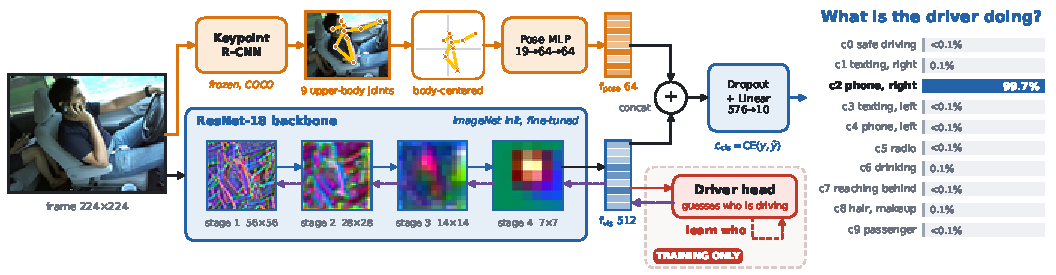
\includegraphics[width=\linewidth]{figures/model.pdf}
  \caption{\textbf{Architecture overview (Configs~\texttt{D-I} and~\texttt{F-I}).}
  A $224 \times 224$ frame passes through a ResNet-18 visual stream (blue) and an optional body-centered pose stream (orange), whose embeddings are concatenated to predict the 10 distraction classes. During training, a driver head attaches to the visual embedding $\mathbf{f}_{\text{vis}}$ to learn driver identity (red dashed arrow) while sending adversarial gradients back into the visual backbone to erase it (purple dashed arrows). See Section~\ref{sec:network} for full details.}
  \label{fig:model}
\end{figure*}


\paragraph{Visual Stream.}
% Source: distracted_driver.ipynb Section 4 (DriverNet), cell 3 settings, table_model_parameters.csv.
We use a ResNet-18~\cite{he2016resnet} backbone operating on $224 \times 224$ ImageNet-normalized RGB frames across four residual stages ($56 \times 56$ to $7 \times 7$). Global average pooling over the final stage yields the visual representation $\mathbf{f}_{\text{vis}} \in \mathbb{R}^{512}$. To test whether pretraining changes how strongly a model memorizes drivers, every configuration is trained both from random initialization (\texttt{-S}) and from ImageNet-1K~\cite{russakovskyImageNet2015} weights (\texttt{-I}).

\paragraph{Body-Centered Pose Stream.}
% Source: distracted_driver.ipynb Section 2 (pose keypoint extraction) and Section 4 (pose MLP).
To supply appearance-free body geometry, we extract 9 upper-body keypoints (nose, ears, shoulders, elbows, and wrists) offline with a frozen COCO Keypoint R-CNN~\cite{he2017maskrcnn} (confidence threshold $0.5$). Raw image coordinates still encode where each driver sits and how large they appear, so we re-express every joint relative to the driver's own shoulders. The origin moves to the midpoint between the shoulders, and one unit equals the shoulder width. Let $\mathbf{k}_j \in [0, 1]^2$ be the image position of joint $j$, with $\mathbf{k}_{\text{ls}}$ and $\mathbf{k}_{\text{rs}}$ the left and right shoulders, respectively, and let $\delta \in \{0, 1\}$ indicate whether a person was detected. With mid-shoulder point $\mathbf{m} = \tfrac{1}{2}(\mathbf{k}_{\text{ls}} + \mathbf{k}_{\text{rs}})$ and shoulder width $w = \max(\|\mathbf{k}_{\text{ls}} - \mathbf{k}_{\text{rs}}\|_2,\, 0.05)$, clamped to avoid dividing by a near-zero width, each joint becomes
\begin{equation}
  \tilde{\mathbf{k}}_j = \delta \, \frac{\mathbf{k}_j - \mathbf{m}}{w},
  \label{eq:pose_norm}
\end{equation}
which is all zeros when no person is detected. Flattening the 9 normalized joints and appending $\delta$ gives a 19-d vector $\mathbf{p} \in \mathbb{R}^{19}$, which a 2-layer Pose MLP ($19 \!\to\! 64 \!\to\! 64$, ReLU) projects to $\mathbf{f}_{\text{pose}} \in \mathbb{R}^{64}$.

\paragraph{Classification Head.}
% Source: distracted_driver.ipynb Section 4 (DriverNet classifier).
The classifier reads $\mathbf{f}_{\text{vis}}$, or $[\mathbf{f}_{\text{vis}};\, \mathbf{f}_{\text{pose}}] \in \mathbb{R}^{576}$ with pose fusion. Dropout ($p = 0.30$) followed by a linear layer outputs class probabilities $\hat{y}$ over the 10 distraction classes, trained with the cross-entropy loss $\mathcal{L}_{\text{cls}} = \mathrm{CE}(y, \hat{y})$, where $\mathrm{CE}(q, p) = -\sum_c q_c \log p_c$ and $y$ is one-hot.

\paragraph{Training-Only Driver Adversary.}
% Source: distracted_driver.ipynb Section 4 (GradReverse, confusion_loss), adversarial_study.ipynb
% Sections 5 and 6 (lambda and ramp, confusion loss).
To remove driver identity from $\mathbf{f}_{\text{vis}}$ at zero test-time cost, we attach a 2-layer MLP driver head $h_d$ ($512 \!\to\! 256 \!\to\! K$, ReLU) during training to predict which of the $K$ training drivers $d$ appears in the frame. Training optimizes two opposing objectives (Fig.~\ref{fig:model}). The head $h_d$ updates only itself to \emph{learn who} is driving by minimizing $\mathrm{CE}(d,\, h_d(\mathbf{f}_{\text{vis}}))$ on detached features, while the backbone updates through a frozen copy of $h_d$ to \emph{hide who} is driving by minimizing one of
\begin{align}
  \mathcal{L}_{\text{GRL}} &= \mathcal{L}_{\text{cls}} - \lambda(p)\,\mathrm{CE}\!\left(d,\, h_d(\mathbf{f}_{\text{vis}})\right),
  \label{eq:grl} \\
  \mathcal{L}_{\text{conf}} &= \mathcal{L}_{\text{cls}} + \lambda(p)\,\mathrm{CE}\!\left(\mathbf{u},\, h_d(\mathbf{f}_{\text{vis}})\right),
  \label{eq:conf}
\end{align}
where $\mathbf{u} \in \mathbb{R}^K$ is the uniform distribution ($1/K$ per driver) and $\lambda(p) = \lambda_{\max}\!\left(\tfrac{2}{1 + \exp(-10p)} - 1\right)$ ramps adversary strength over training progress $p \in [0, 1]$ up to $\lambda_{\max} = 1.0$ via the domain-adversarial (DANN) schedule~\cite{ganin2016dann} (selected in Sec.~\ref{sec:robustness}). Gradient reversal (GRL, Eq.~\ref{eq:grl})~\cite{ganin2016dann} flips the gradient sign so the backbone maximizes driver error; because negative cross-entropy is unbounded, the backbone can cheat by making $h_d$ confidently wrong rather than uncertain. Confusion loss (Eq.~\ref{eq:conf})~\cite{tzeng2015confusion,alvi2018turning} fixes this by pushing $h_d$ toward a uniform guess, a bounded target reached only when $\mathbf{f}_{\text{vis}}$ carries no usable driver cues. At each step, $h_d$ chases any remaining identity signal while the backbone's adversarial gradient (purple arrows in Fig.~\ref{fig:model}) strips it out across all four ResNet stages.

% Placed where the text has reached page 3's right column, so it floats to the top of
% that column under Fig. 1.
\begin{table}[t]
  \centering
  \small
  \caption{\textbf{Model ablation ladder.} Every row is trained both from
  scratch (\texttt{-S}) and from ImageNet-1K weights (\texttt{-I}).}
  \label{tab:ablation_ladder}
  \begin{tabular}{@{}llcc@{}}
    \toprule
    ID & Configuration & Driver Adversary & Pose Fusion \\
    \midrule
    \texttt{A} & Baseline & --- & --- \\
    \texttt{B} & + GRL adversary & GRL & --- \\
    \texttt{C} & + Pose fusion & --- & \checkmark \\
    \texttt{D} & Full GRL & GRL & \checkmark \\
    \texttt{E} & + Confusion adversary & Confusion & --- \\
    \texttt{F} & Full Conf. & Confusion & \checkmark \\
    \bottomrule
  \end{tabular}
\end{table}

\paragraph{Ablation Ladder.}
% Source: distracted_driver.ipynb Section 6.2 (configurations).
Our ablation ladder (Table~\ref{tab:ablation_ladder}) is six models that each add or swap one component, trained under both initializations (12 models). Comparing \texttt{B} vs.\ \texttt{E} and \texttt{D} vs.\
\texttt{F} isolates the adversarial objective, while comparing \texttt{D} and
\texttt{F} against \texttt{C} isolates what identity removal adds once pose is
present.

%-------------------------------------------------------------------------
\subsection{Training Details}
% Source: distracted_driver.ipynb cell 3 settings.
All convolutional models train on $224 \times 224$ RGB frames for 15 epochs (batch size 64) using AdamW~\cite{loshchilovAdamW2019} (weight decay $10^{-4}$), a OneCycleLR schedule~\cite{smithSuperconvergence2019}, and CUDA automatic mixed precision. Peak learning rates are $10^{-3}$ for from-scratch backbones and newly initialized heads, and $3 \times 10^{-4}$ for ImageNet-pretrained backbones. Augmentation is limited to random brightness and contrast jitter ($\pm 15\%$). Label-consistent horizontal flips (swapping left/right phone and texting classes) were tested separately and excluded. A mirrored frame shows a right-hand-drive cabin seen from the opposite side, a viewpoint that never occurs in the dataset and is rare in practice, and the flip lowered cross-validation accuracy (0.855 to 0.845 for \texttt{A-I}, 0.507 to 0.444 for \texttt{A-S}). Remaining hyperparameters (dropout $p = 0.3$, keypoint confidence threshold 0.5, learning rates, and epoch count) follow common defaults and were fixed before the experiments rather than tuned, so all configurations share identical settings. To avoid unequal tuning, every model uses fixed seed~42, plus fresh multi-seed runs for adversarial confirmation, and is evaluated strictly from its final-epoch weights without early stopping; hardware, precision settings, compute budget, and code attribution appear at the end of the paper.

\section{Experiments}
\label{sec:experiments}

% Budget: about 1.5 column-pages. This section carries required components 1 to 4.
% Rubric (4 pts): appropriate metrics, defended, comparison to the state of the art qualified.
% Source: distracted_driver.ipynb Section 6.1 (table_folds.csv) and Section 5.2 (driver probe).

We evaluate every model with 3-fold driver-grouped cross-validation and then score it once on the 4 frozen test drivers (Sec.~\ref{sec:data}). We report the cross-validation mean $\pm$ standard deviation alongside the test result. To measure how much driver identity survives in a network's visual features, we use a \emph{driver probe}, a separate classifier trained to guess which unseen driver appears in a frame from the model's frozen last-stage features. The probe is trained on classes \texttt{c0}--\texttt{c4} and tested on \texttt{c5}--\texttt{c9}, then the reverse. Frames from one video burst are nearly identical, so without this class split the probe could match a test frame to its near-duplicate in training instead of recognizing the driver. Lower probe accuracy means less driver identity remains.

%-------------------------------------------------------------------------
\subsection{Driver Leakage in Random Splits}
\label{sec:leakage}
% Source: Section 7, table_leakage_study.csv, table_leakage_group_split.csv, fig05.
A naive random frame split severely inflates performance on SFDDD (Table~\ref{tab:leakage_classical}). Because near-identical frames from the same video burst land in both training and validation, every model approaches ceiling accuracy under random splitting. Even the from-scratch CNN (\texttt{A-S}) and purely classical \texttt{HOG + RF} exceed 99\%. Under driver-disjoint folds, performance collapses sharply. \texttt{A-S} falls by 49.0 points ($0.997 \!\to\! 0.507$), \texttt{HOG + RF} drops by 40.4 points, and even ImageNet-pretrained \texttt{A-I} loses 14.3 points. Random-split scores therefore measure driver and cabin memorization rather than distraction recognition.

%-------------------------------------------------------------------------
\subsection{Classical Baselines versus CNNs}
\label{classical}
% Source: Section 12, Table/Figure 17.
% Where HOG + RF sits between A-S and A-I on unseen drivers. Whether body-centering helps
% the pose forest. What the deep network actually buys.
Comparing against non-neural classifiers shows what end-to-end convolutional learning actually adds (Table~\ref{tab:leakage_classical}). Hand-crafted HOG features generalize poorly to unseen drivers (0.590), yet they still beat the from-scratch CNN (0.507 for \texttt{A-S}), which overfits to cabin details when trained on only 14--15 drivers. Pose features do much better. A Random Forest on the 19 body-centered pose features reaches $0.795 \pm 0.011$, ahead of the same forest on raw image-centered keypoints (0.765) and of every from-scratch CNN, including \texttt{F-S} (0.693). Centering the keypoints on the shoulders removes seat position and body size before learning begins. ImageNet-pretrained CNNs are still the strongest overall, with 0.855 for \texttt{A-I} and 0.873 for \texttt{F-I} (0.927 on the test drivers). Where the pose forest sees only 9 upper-body joints, their visual features can tell apart the small objects that separate many classes, such as phones, cups, and cosmetics. 

% Placed where the text has reached page 4's right column, so it floats to the top of
% that column.
\begin{table}[t]
  \centering
  \small
  \caption{\textbf{Driver leakage and classical vs.\ CNN baselines.} Accuracy
  on a random frame split versus 3-fold driver-grouped cross-validation; the gap quantifies
  inflation from seeing the same drivers in training and validation.}
  \label{tab:leakage_classical}
  \setlength{\tabcolsep}{4pt}
  \begin{tabular}{@{}lccc@{}}
    \toprule
    Model & Random & Driver-grouped & Gap \\
    \midrule
    \texttt{A-S} (CNN, scratch) & 0.997 & $0.507 \pm 0.059$ & 0.490 \\
    \texttt{A-I} (CNN, ImageNet) & 0.997 & $0.855 \pm 0.051$ & 0.143 \\
    \texttt{HOG + RF} & 0.994 & $0.590 \pm 0.068$ & 0.404 \\
    \texttt{Pose (image) + RF} & 0.969 & $0.765 \pm 0.044$ & 0.205 \\
    \texttt{Pose (body) + RF} & 0.944 & $0.795 \pm 0.011$ & 0.149 \\
    \bottomrule
  \end{tabular}
\end{table}

% Full-width floats appear one page after their source, so this sits early to land on page 5.
\begin{table*}[t]
  \centering
  \small
  \caption{\textbf{Main ablation results.} Performance across 3-fold driver-grouped cross-validation (mean $\pm$ standard deviation over folds) and a single run on the four frozen test drivers. Models are initialized either from scratch (\texttt{-S}) or from ImageNet weights (\texttt{-I}). Probe is the driver probe defined in Sec.~\ref{sec:experiments}, where lower values indicate less driver identity (cross-validation chance is 0.137).}
  \label{tab:ablation_results}
  \setlength{\tabcolsep}{4pt}
  % Generated by figures/make_ablation_table.py from outputs/main/table_summary.csv and
% outputs/main/table_final_test.csv. Do not edit by hand, rerun the script instead.
\begin{tabular}{@{}llcccccccc@{}}
    \toprule
    & & \multicolumn{4}{c}{3-Fold Driver-Grouped Cross-Validation} & \multicolumn{4}{c}{Frozen Test (4 Drivers)} \\
    \cmidrule(lr){3-6} \cmidrule(l){7-10}
    ID & Configuration & Acc & Macro-F1 & Log-Loss & Probe & Acc & Macro-F1 & Log-Loss & Probe \\
    \midrule
    \texttt{A-S} & Baseline & $0.507 \pm 0.059$ & $0.505 \pm 0.054$ & $2.099 \pm 0.569$ & $0.796 \pm 0.054$ & $0.627$ & $0.609$ & $2.152$ & $0.715$ \\
    \texttt{B-S} & + GRL & $0.520 \pm 0.079$ & $0.522 \pm 0.082$ & $1.833 \pm 0.486$ & $0.823 \pm 0.040$ & $0.712$ & $0.696$ & $1.403$ & $0.789$ \\
    \texttt{C-S} & + Pose & $0.526 \pm 0.034$ & $0.527 \pm 0.028$ & $1.882 \pm 0.412$ & $0.827 \pm 0.028$ & $0.715$ & $0.694$ & $1.228$ & $0.677$ \\
    \texttt{D-S} & Full GRL & $0.544 \pm 0.097$ & $0.542 \pm 0.078$ & $1.770 \pm 0.633$ & $0.836 \pm 0.025$ & $\mathbf{0.734}$ & $\mathbf{0.709}$ & $1.255$ & $0.738$ \\
    \texttt{E-S} & + Confusion & $0.501 \pm 0.028$ & $0.503 \pm 0.042$ & $1.522 \pm 0.067$ & $\mathbf{0.668 \pm 0.041}$ & $0.675$ & $0.658$ & $1.125$ & $\mathbf{0.624}$ \\
    \texttt{F-S} & Full Conf.\ & $\mathbf{0.693 \pm 0.087}$ & $\mathbf{0.683 \pm 0.082}$ & $\mathbf{0.859 \pm 0.102}$ & $0.746 \pm 0.077$ & $0.713$ & $0.678$ & $\mathbf{0.844}$ & $0.723$ \\
    \midrule
    \texttt{A-I} & Baseline & $0.855 \pm 0.051$ & $0.853 \pm 0.051$ & $0.488 \pm 0.182$ & $0.713 \pm 0.073$ & $0.934$ & $0.923$ & $0.408$ & $0.558$ \\
    \texttt{B-I} & + GRL & $0.862 \pm 0.057$ & $0.859 \pm 0.057$ & $0.475 \pm 0.157$ & $0.589 \pm 0.100$ & $0.906$ & $0.883$ & $0.457$ & $0.551$ \\
    \texttt{C-I} & + Pose & $0.845 \pm 0.048$ & $0.842 \pm 0.048$ & $0.516 \pm 0.194$ & $0.585 \pm 0.069$ & $\mathbf{0.942}$ & $\mathbf{0.932}$ & $0.368$ & $0.561$ \\
    \texttt{D-I} & Full GRL & $\mathbf{0.874 \pm 0.038}$ & $0.870 \pm 0.038$ & $0.456 \pm 0.095$ & $0.550 \pm 0.071$ & $0.914$ & $0.899$ & $0.415$ & $0.636$ \\
    \texttt{E-I} & + Confusion & $0.856 \pm 0.057$ & $0.854 \pm 0.060$ & $0.502 \pm 0.159$ & $\mathbf{0.315 \pm 0.033}$ & $0.874$ & $0.870$ & $0.431$ & $\mathbf{0.379}$ \\
    \texttt{F-I} & Full Conf.\ & $0.873 \pm 0.021$ & $\mathbf{0.871 \pm 0.021}$ & $\mathbf{0.407 \pm 0.024}$ & $0.396 \pm 0.032$ & $0.927$ & $0.917$ & $\mathbf{0.286}$ & $0.389$ \\
    \bottomrule
\end{tabular}

\end{table*}

%-------------------------------------------------------------------------
\subsection{Ablation of the Adversary and Pose Fusion}
% Source: Sections 8.1 and 8.6, table_ablation_summary.csv, table_ablation_deltas.csv, fig16_ablation_summary.
% Main results table: CV accuracy, macro-F1, log-loss, probe (mean and std over folds) and
% test accuracy and macro-F1 for A to D, both initializations, plus the classical rows.
% Read every difference against the fold std and the "helped in k of 3 folds" count.
Three clear patterns emerge across the 12-model ablation ladder (Table~\ref{tab:ablation_results}). First, erasing driver identity \emph{alone} does not improve action recognition. Adding the confusion adversary leaves cross-validation macro-F1 essentially flat on both ImageNet and from-scratch runs, while ImageNet gradient reversal adds less than a point. Second, pairing the bounded confusion loss with body-centered pose fusion (\texttt{F-I}) outperforms either component alone. On ImageNet, \texttt{F-I} reaches the highest cross-validation macro-F1 at 0.871, gaining 1.8 points over the visual baseline and 2.9 points over pose alone, and the lowest log-loss at 0.407, while matching full GRL's accuracy with roughly half the fold-to-fold standard deviation ($\pm 0.021$ vs.\ $\pm 0.038$ for \texttt{D-I}, and under half that of all other ImageNet models). Finally, this balance holds on the four frozen test drivers, where \texttt{F-I} achieves 0.927 accuracy and 0.917 macro-F1 alongside the best probability calibration of any model (0.286 log-loss vs.\ 0.408 for the baseline), while cutting the driver probe to 0.389, well below both the baseline and full GRL.

\paragraph{ImageNet Pretraining versus From Scratch.}
% Source: distracted_driver.ipynb Section 10, table_init_comparison.csv,
% table_init_paired_delta.csv, table_results_per_fold.csv.
ImageNet initialization provides the single largest gain on unseen drivers. It raises cross-validation accuracy by 34.8 points over training from scratch (\texttt{A-I} vs.\ \texttt{A-S}) and shrinks the leakage drop from 49.0 to 14.3 points (Table~\ref{tab:leakage_classical}), since pretrained features keep a ResNet-18 from overfitting cabin textures on 14--15 drivers. Without pretraining, the confusion loss and pose fusion together close about half of that gap. The full from-scratch model (\texttt{F-S}) gains 18.6 points of accuracy over \texttt{A-S} ($0.507 \!\to\! 0.693$), cuts log-loss by more than half ($2.099 \!\to\! 0.859$), and beats every other from-scratch model in all 3 folds. It still trails ImageNet fine-tuning and the body-centered \texttt{Pose + RF}, however.

%-------------------------------------------------------------------------
\subsection{Scaling with the Number of Training Drivers}
\label{sec:scaling}
% Source: Section 11, scaling table, fig14_scaling.
% Answer both questions the instructions ask in one sentence each.
%   Where does it saturate? (or say it has not saturated at 22 drivers)
%   What would more data be worth? (the gain from the last step, with its spread)
% Whether D beats A when drivers are scarce.
\begin{figure*}[t]
  \centering
  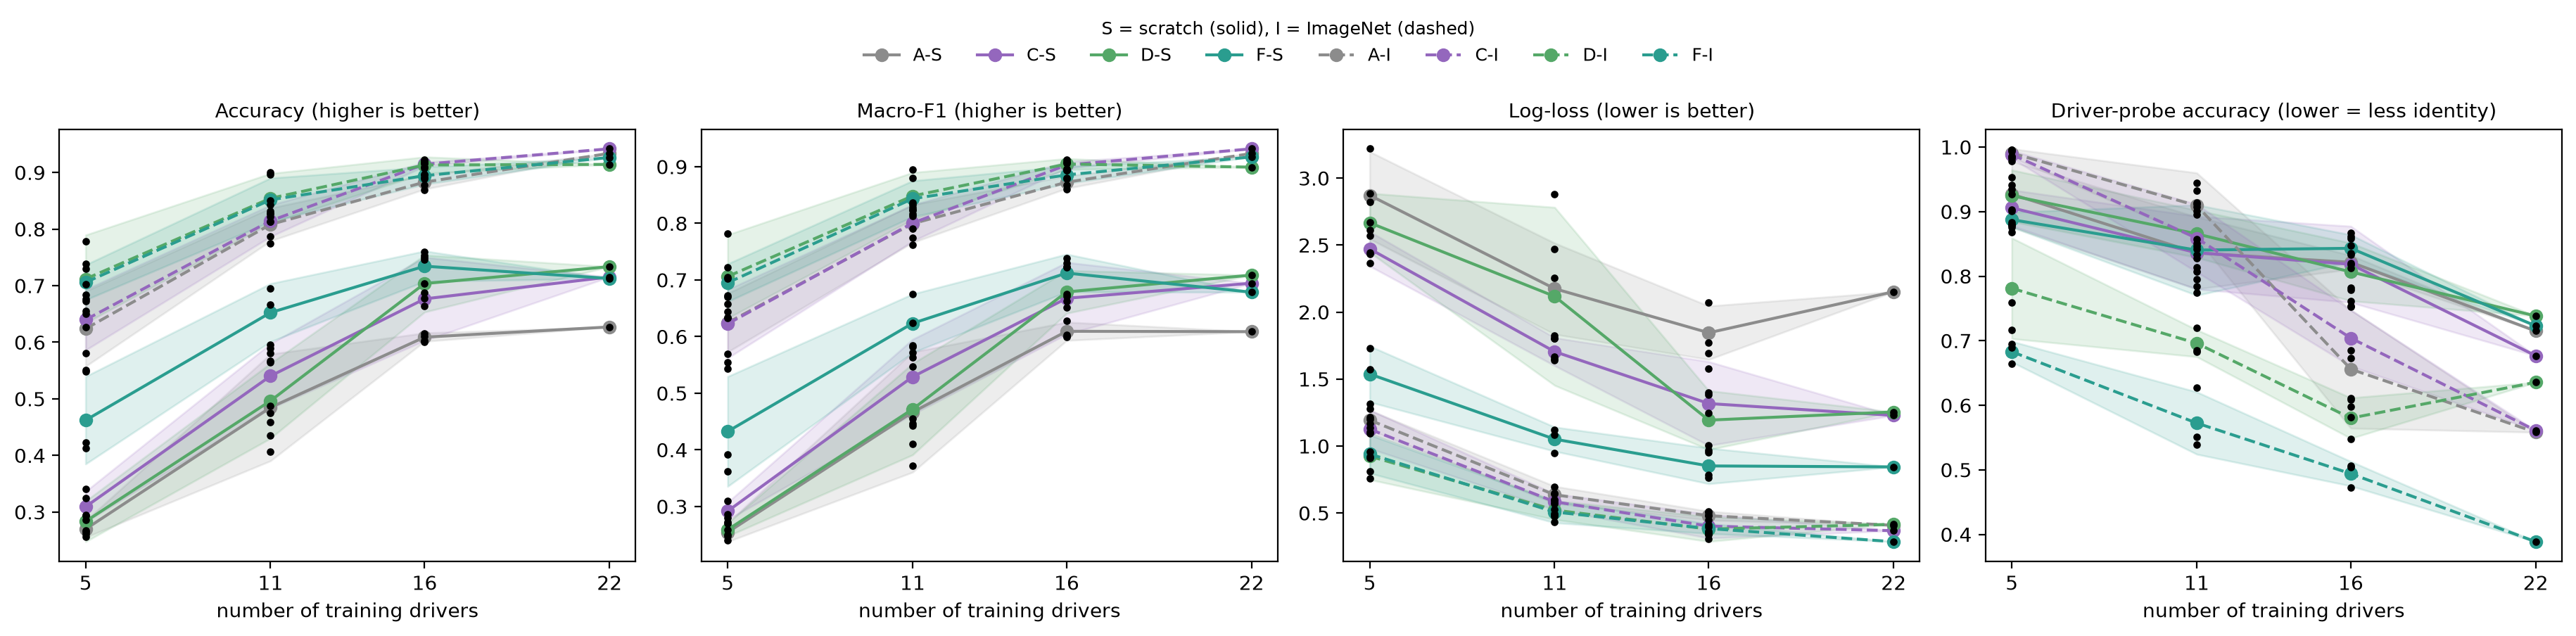
\includegraphics[width=\linewidth]{figures/fig14_scaling.png}
  \caption{\textbf{Scaling with the number of training drivers.} Test-driver accuracy, macro-F1, log-loss, and driver-probe accuracy for \texttt{A}, \texttt{C}, \texttt{D}, and \texttt{F}, from scratch (solid) and ImageNet (dashed). We omit \texttt{B} and \texttt{E} to limit compute, since Table~\ref{tab:ablation_results} shows that removing identity alone barely changes accuracy. Lines show means over random driver subsets, shaded bands one standard deviation, and dots individual runs (22 drivers is the single final model from Table~\ref{tab:ablation_results}).}
  \label{fig:scaling}
\end{figure*}

Figure~\ref{fig:scaling} tracks frozen-test performance as the training pool grows from 5 to 22 drivers (25\%--100\% of the development set). Pose fusion and adversarial regularization help most when driver diversity is scarce. With only 5 training drivers, the ImageNet baseline memorizes identity almost completely (0.991 probe) and falls to 0.624 test accuracy. Under the same 5-driver regime, combining pose fusion with an adversary lifts ImageNet accuracy by more than 8 points, reaching 0.712 with GRL and 0.706 with confusion loss (\texttt{F-I}), which also halves the run-to-run standard deviation and lowers the probe to 0.683. The gain is even starker from scratch, where \texttt{F-S} nearly doubles baseline accuracy (0.462 vs. 0.270). Although accuracy gaps narrow by 16 drivers, \texttt{F-I} retains a steady 0.16--0.34 probe advantage at every training size. Performance has not saturated at 22 drivers. Moving from 16 to 22 drivers still adds 5.1 points for the baseline and 3.3 points for \texttt{F-I}, so additional training drivers would likely improve accuracy further.

%-------------------------------------------------------------------------
\subsection{Adversary Design and Robustness}
\label{sec:robustness}
% Sources: Section 8.5 (table_final_test.csv, per-test-driver accuracy, fig15), Section 8.2 (fig10 driver probe), Section 9 (fig12).
% Spread of accuracy across the four test drivers. Whether the adversary lowers the probe.
% The adversarial study (adversarial_study.ipynb) goes here in one or two sentences, with
% details in the supplementary material.
To diagnose why standard gradient reversal (\texttt{B-I}) barely reduced driver identifiability in Table~\ref{tab:ablation_results}, and to choose our final adversary without touching the test set, we screened candidate designs on ImageNet ResNet-18 (Fold~0). Each candidate was scored with the worst case of class-split linear and MLP driver probes. Promising designs and mechanism checks were then confirmed with fresh multi-seed runs on 3 and 5-fold driver-grouped cross-validation
(Table~\ref{tab:adv_ablation}).

\begin{table}[t]
  \centering
  \small
  \caption{\textbf{Adversarial design ablation (ImageNet ResNet-18).} Screening rows report the Fold~0 worst-case linear/MLP driver probe, where lower is better, and macro-F1. On Fold~0, chance is 0.143 and always guessing the most common driver scores 0.195 (the majority floor). Untrained anchors use the hardened multi-split probe on 5 folds, and 5-fold confirmation rows average fresh seeds (chance 0.230).}
  \label{tab:adv_ablation}
  \setlength{\tabcolsep}{4pt}
  \begin{tabular}{@{}llcc@{}}
    \toprule
    Stage & Variant & Probe & Macro-F1 \\
    \midrule
    \multicolumn{4}{@{}l}{\textit{Untrained anchors (5-fold multi-split probe)}} \\
    Anchor & Random init & 0.999 & --- \\
    Anchor & Frozen ImageNet & 1.000 & --- \\
    \midrule
    \multicolumn{4}{@{}l}{\textit{Fold-0 screening (single-factor changes)}} \\
    Ref. & Baseline (no adversary) & 0.627 & 0.881 \\
    Ref. & GRL ($\lambda{=}1$, DANN ramp) & 0.607 & 0.884 \\
    Head & GRL, 2 head steps & 0.547 & 0.880 \\
    Strength & GRL, $\lambda{=}10$ & 0.577 & 0.876 \\
    Loss & Confusion, $\lambda{=}1$ (last stage) & \textbf{0.388} & 0.868 \\
    Loss & Confusion, $\lambda{=}3$ (last stage) & 0.333 & 0.841 \\
    Stages & Conf.\ $\lambda{=}3$, last 2 stages & 0.375 & 0.790 \\
    \midrule
    \multicolumn{4}{@{}l}{\textit{Mechanism, post-hoc, and 5-fold confirmation}} \\
    Mech. & GRL ensemble + head resets & 0.809 & --- \\
    Post-hoc & Baseline + forced INLP & 0.593 & --- \\
    \mbox{5-fold} & Baseline, no pose & 0.674 & 0.860 \\
    \mbox{5-fold} & Confusion $\lambda{=}1$, no pose & \textbf{0.446} & 0.857 \\
    \mbox{5-fold} & Confusion $\lambda{=}1$ + pose & 0.450 & \textbf{0.878} \\
    \bottomrule
  \end{tabular}
\end{table}

\paragraph{Baseline Identity Levels and Why GRL Fails.}
% Source: adversarial_study.ipynb Sections 3, 4, 5, 11 (outputs/adversarial/table_s3_anchors.csv,
% table_s3_reference.csv, table_s4_head.csv, table_s5_lambda.csv, table_s11_ensemble.csv).
Before fine-tuning, both frozen ImageNet and randomly initialized ResNet-18 features identify held-out drivers nearly 100\% of the time across disjoint action classes (Table~\ref{tab:adv_ablation}), showing that raw color and cabin textures uniquely fingerprint each subject. Standard fine-tuning lowers the driver probe to 0.627 on Fold~0 and 0.674 across 5 folds. Gradient reversal does only slightly better. Across deeper heads, $3\times$ head learning rates, extra head updates, penalty weights up to $\lambda{=}10$, constant ramps, multi-stage heads, and ensembles, the probe never drops below 0.547, and periodically resetting the head makes it worse (0.809). The cause is that gradient reversal rewards making the driver head wrong, not uncertain. The backbone learns to make the head confidently pick the wrong driver, so the head itself is right only 9.5\% of the time. The identity is still present, just relabeled, and a fresh linear probe trained on the same features still names the training drivers 67.7\% of the time.

\paragraph{Bounded Confusion Loss and Alternatives.}
% Source: adversarial_study.ipynb Sections 6, 7, 8, 12, 13, 14, 15 (table_s6_confusion.csv,
% table_s7_stages.csv, table_s8_augmentation.csv, table_s12_extended.csv, table_s13_inlp.csv,
% table_s14_probe_hardening.csv, table_s15_confirm5.csv, table_s15_hardened.csv).
Switching from GRL to the bounded uniform confusion loss ($\lambda{=}1$) on
the last stage resolves this failure mode. A uniform guess is the best the backbone
can reach, so it has no reason to make the head confidently wrong. On Fold~0, it cuts the driver probe to
0.388 while keeping macro-F1 within 0.02 of the baseline, whereas stronger penalties
($\lambda{=}3$) or earlier-stage heads degrade macro-F1
(Table~\ref{tab:adv_ablation}). Confirmed across 5 folds with fresh seeds,
last-stage confusion loss drives training-driver identity down to chance and cuts
the held-out probe by 22.8 points (0.446 vs.\ 0.674). That removes
over 60\% of the driver identity signal above the majority-class floor while
leaving macro-F1 virtually unchanged (0.857 vs.\ 0.860). Stricter checks using
multi-split, wide MLP, and $k$-NN probes show matching drops, confirming that
driver cues are genuinely erased rather than merely hidden from a linear
classifier. Finally, non-adversarial alternatives fall short. Neither heavy
appearance augmentation nor projecting out driver directions after training
via Iterative Nullspace Projection (INLP, 0.593) matches confusion
training.

% Placed where the text has reached page 6's right column, so it floats to the top of
% that column on the same page as the SOTA section.
\begin{table}[t]
  \centering
  \footnotesize
  \caption{\textbf{Comparison with published SFDDD methods by split protocol.} All rows evaluate on SFDDD; because held-out driver subsets vary across papers, scores are not directly comparable. NLL denotes multi-class log-loss where reported.}
  \label{tab:sota}
  \setlength{\tabcolsep}{3.5pt}
  \begin{tabular}{@{}llcc@{}}
    \toprule
    Method & Split Protocol & Acc & NLL $\downarrow$ \\
    \midrule
    \multicolumn{4}{@{}l}{\textit{Random frame splits (driver leakage)}} \\
    ViT-DD~\cite{ma2024vitdd} & Random (70/30) & 0.996 & 0.017 \\
    Ours (\texttt{A-I}, naive) & Random (67/33) & 0.997 & 0.013 \\
    \midrule
    \multicolumn{4}{@{}l}{\textit{Driver-disjoint splits (unseen drivers)}} \\
    Hssayeni \etal~\cite{hssayeni2017} (ResNet-152) & Driver-disj. & 0.850 & --- \\
    MobileNetV3-L~\cite{essahraui2026} & Driver-disj. & 0.889 & --- \\
    DEWS-EfficientNet~\cite{zhangCrossDriver} & Driver-disj. & 0.890 & --- \\
    Anchor-ViT~\cite{doshiAnchorVIT} & SFDDD val.$^\star$ & 0.923 & --- \\
    ViT-DD~\cite{ma2024vitdd} & Driver-disj.\ (18/6) & 0.925 & 0.397 \\
    Ours (\texttt{F-I}) & 3-fold driver-disj. & 0.873 & 0.407 \\
    Ours (\texttt{F-I}) & Driver-disj.\ (22/4) & 0.927 & 0.286 \\
    \bottomrule
    \multicolumn{4}{@{}l}{\scriptsize $^\star$Validation accuracy (92.4\% F1).}
  \end{tabular}
\end{table}

\paragraph{Effect on Unseen-Driver Robustness.}
% Source: adversarial_study.ipynb Sections 15, 16, 17 (table_s15_pose5.csv, table_s15_pose_fcls.csv,
% table_s16_test_delta.csv, table_s17_decoupling.csv), distracted_driver.ipynb Section 8.3b
% (table_error_by_driver.csv).
Across 105 visual-only 5-fold runs, lower driver identifiability alone does
not predict higher macro-F1 (slope $+0.036$, 95\% CI $[-0.016, +0.069]$). Its
practical payoff emerges when paired with pose fusion and on the hardest
unseen subjects. Across 5 folds, confusion loss plus pose cuts the visual
driver probe by 22.3 points to 0.450 while lifting macro-F1 by 1.8 points to
0.878 over the visual baseline (95\% CI $[+0.008, +0.027]$). On the four
frozen test drivers across three seeds, it lowers the driver probe by 13.1
points (0.420 vs.\ 0.551) and cuts log-loss by 0.115 (0.309 vs.\ 0.424) at
$0.917 \pm 0.002$ macro-F1. Most notably, in the main study \texttt{F-I} cuts
error rates on the two hardest development drivers (\texttt{p072} and
\texttt{p081}) by 27.2 and 25.6 points relative to the visual
baseline.

%-------------------------------------------------------------------------
\subsection{Comparison to the State of the Art}
\label{sec:sota}
% Source: published numbers from the cited papers (see Sec. 2). Our rows from
% table_leakage_study.csv, table_summary.csv, and table_final_test.csv.

Table~\ref{tab:sota} compares our final model against representative SFDDD
benchmarks grouped by split protocol. Because studies differ in held-out
drivers and fold schemes, absolute accuracies are \emph{not} directly
comparable across papers, and we do not claim to beat the state of the art.

Under random frame splits, published SFDDD models routinely exceed 99\%
accuracy (e.g., ViT-DD~\cite{ma2024vitdd} at 99.6\%, CAT-CapsNet~\cite{mittal2023catcaps}
at 99.9\%), matching our naive ImageNet baseline (\texttt{A-I}, 99.7\%) and
confirming that random splits primarily measure driver leakage
(Sec.~\ref{sec:leakage}). Under driver-disjoint splits, published accuracy
drops to 85--92.5\%. Transfer-learned ResNet-152~\cite{hssayeni2017} sits at
85.0\% (matching our \texttt{A-I} cross-validation baseline at 85.5\%), while recent
unseen-driver CNNs~\cite{zhangCrossDriver,essahraui2026} reach $\sim$89\%. The
highest scores come from heavier Vision Transformers that localize upper-body
or facial cues. Anchor-ViT~\cite{doshiAnchorVIT} reaches 92.3\% via learned
spatial anchors, and ViT-DD~\cite{ma2024vitdd} reaches 92.5\% (0.397 NLL) via
face crops and multi-task emotion labels. Our \texttt{F-I} model achieves
competitive accuracy and strong calibration (0.873 accuracy and 0.407 log-loss in cross-validation,
0.927 and 0.286 on test) on a single ResNet-18 backbone by pairing 19-d
body-centered pose fusion with a training-only uniform confusion loss,
complementing recent camera-view disentanglement work~\cite{celona2026dbmnet}
by directly erasing and verifying driver invariance.

\section{Error Analysis}
\label{sec:errors}

% Budget: about 0.8 column-pages plus one figure. Rubric: 5 pts, the largest report item.
% "Real failure cases shown, patterns identified, explanations proposed."
% Sources: Section 8.3b (fig11b_error_corrected, fig11c_error_persistent,
% table_error_pairs.csv, table_error_by_class.csv, table_error_by_driver.csv),
% Section 8.3 (fig11_gradcam), Section 8.1 (fig09 confusion matrices, fig08 per-class F1).
% Structure:
%   1. Overall error rate of the final model and the top confusion pairs with counts.
%   2. A figure of real failure frames with Grad-CAM (persistent mistakes, plus 1 or 2
%      corrected ones). Check data use rules before showing frames.
%   3. Name each pattern and give a proposed cause (for example c0 vs. c9 differ only by a
%      small head turn, c8 shares the raised hand with the phone classes).
%   4. Per-driver concentration (the worst drivers) and a proposed cause, marked as a
%      hypothesis unless checked.
%   5. Where the full model helps and where it hurts the baseline (frames fixed vs. broken).
% The paragraphs below are the earlier draft from the first model. Replace the numbers with
% the final model's numbers, and replace the figure with fig09 or fig15.

Error analysis included metrics not previously shown for the model to help better determine accuracy, bias, as well as allow us to be able to determine the best modifications for finetuning.
New statistics included: entropy loss, F1 precision, and total accuracy. These were accomplished by using sklearn metrics to be computed after and during the model.

Originally, the model did not fair the best with an accuracy of 51.8\%.
Recall was the highest with the driver operating the radio at 0.91, and steadily declined from mid 0.6 in makeup, texing, and reaching behind range down to 0.16 when talking to the passenger.
Based on how similar some of the poses are such as texting and using the phone, the recall is a significantly higher due to the clusters it creates by similarity.

The largest issue that can be denoted from this data is the inability to generalize new drivers.
Not only is this denoted in the accuracy, but the high cross entropy.

\begin{figure}[t]
  \centering
    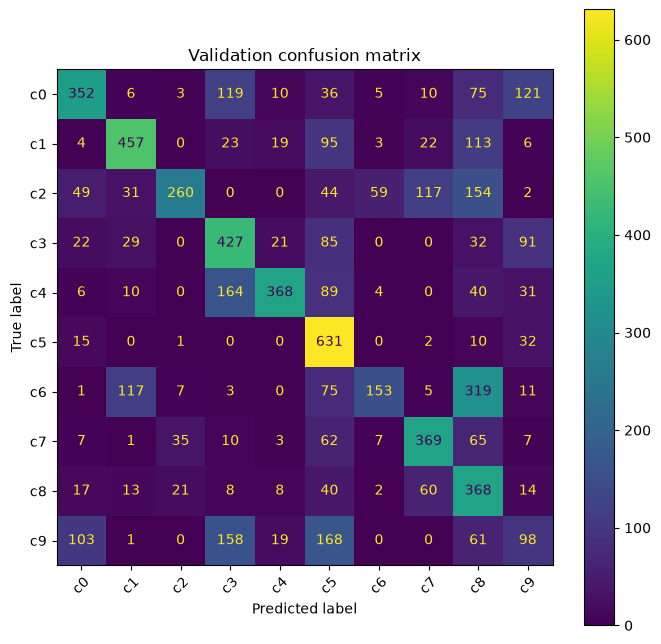
\includegraphics[width=\linewidth]{figures/Val_Conf_Matrix.png}
    \caption{Original confusion matrix after training.}
    \label{ffig:confmat}
  \hfill
\end{figure}

\TODO{Failure-case figure with Grad-CAM, named patterns, and proposed causes.}

\section{Discussion and Limitations}
\label{sec:discussion}

% Budget: about 0.35 column-pages. Rubric (2 pts): "what would improve performance, and why.
% Negative results included" (R10).

What we could to do improve the model.

% Negative results. Each one says what we tried, what happened, and why we think so:
%   the label-consistent flip (excluded, distracted_driver.ipynb Section 3, fixed camera so a
%   mirrored cabin never occurs at test time), the adversary if it does not lower the probe,
%   pose fusion if it does not help with ImageNet weights.
% What would improve performance and why: more drivers (from the scaling curve), a stronger
%   or multi-stage adversary (adversarialStudy.ipynb), temporal context from video, head pose.
% Limitations: 26 drivers, a 4-driver test set, 3 folds with large spread, a single seed in the
%   main study, final-epoch weights, no hyper-parameter search.
\TODO{Negative results, improvements with reasons, and limitations.}

\section{Conclusion}
\label{sec:conclusion}

% Budget: about 0.15 column-pages. Answer the research question from the introduction in
% 3 or 4 sentences, with the headline test number and the main finding.

Final conclusions.

\TODO{Answer the research question in 3 or 4 sentences.}

% Unnumbered closing statements. Keep each to a few sentences so they fit the page budget.

\section*{Reproducibility and Compute}
% R9. Source: README.md, pyproject.toml and uv.lock, distracted_driver.ipynb Section 13 and
% adversarialStudy.ipynb Section 12 (compute tables).
% Repository URL, environment (Python 3.12, uv), seed 42, the notebooks to run in order,
% hardware (RTX 5070 Ti Laptop GPU), GPU-hours for training, one-time pose extraction, and
% CPU hours for the classical models.
\TODO{Repository link, environment, seeds, hardware, and GPU-hours.}

\section*{Codebase and Attribution}

Early data-loading and ResNet fine-tuning boilerplate referenced two Kaggle
educational notebooks for this competition~\cite{pintelasLab6,pintelasLab7}.
The pipeline evaluated in this paper was rewritten from scratch on top of
\texttt{torchvision} model architectures and pretrained weights, including the
driver-disjoint split protocol, classical and pose-based baselines,
body-centered pose fusion, domain-adversarial heads (gradient reversal and
uniform confusion loss), identity probes, and scaling and error analyses.

\section*{AI Tool Disclosure}
% R11. Required. Omitting it counts as academic dishonesty. Name the tools and what they were
% used for (code, debugging, writing or editing text, figures). Keep it factual.
% The notebooks already carry this notice. Edit the wording below so it matches what the
% team actually did, including any use for the report text.
Generative AI tools were used as coding assistants in preparing the code for this project.
The authors reviewed all AI-assisted code and text and take responsibility for its correctness and for the reported results including: Claude, Gemini, and Cursor.

{
    \small
    \nocite{maDigitalTwin2024, xiongDrivingBehavior2026, tranDeepLDriving2018}
    \bibliographystyle{ieeenat_fullname}
    \bibliography{main}
}

% WARNING: do not forget to delete the supplementary pages from your submission 
% \clearpage
\setcounter{page}{1}
\maketitlesupplementary

% The instructions do not say the supplement will be read, so every required component must
% have its main evidence in the paper body. Put only extra detail here.

\section{Adversarial Identity-Removal Study}
\label{sec:suppl-adv}
% Source: adversarialStudy.ipynb, outputs_adv/ tables S1 to S10 and the figures.
% Protocol (screening on one fold, confirmation on all folds with fresh seeds, paired 95% CIs,
% macro-F1 guardrail), what was tried (stronger head, strength and ramp, confusion loss,
% multi-stage, strong augmentation, stacks), and the result as measured.
\TODO{Adversarial study protocol and results.}

\section{Identity Removal over Training}
% Source: distracted_driver.ipynb Section 9, fig12 (ImageNet) and fig12b (from scratch).
\TODO{t-SNE and probe-over-epochs figures.}

\section{Additional Results}
% Per-fold table (table_results_per_fold.csv), training curves (fig07), per-class F1 (fig08),
% pose detection rate, model sizes, per-class test report (classification_report.txt).
\TODO{Per-fold results, training curves, and per-class tables.}


\end{document}
